%!TEX root = report.tex
In this section we will discuss the control flow in the front end upon certain actions of the user. To avoid a lengthy report we will only discuss the flow of successful cases.

\subsection{Log In}
\label{ss:1:login}
	As mentioned earlier users have to log in to a social network before being allowed to stalk somebody on that network. Since we store the ID of the user and we have not implemented an api call that adds for example the LinkedIn identification to a user that we have already stored with its Facebook identification.

	\Cref{fig:1:controlflowLogIn} presents the flow of control when a users logs in.

	The \t{loggedIn}, and its not shown equivalent \t{loggedOut}, event ensure that the \t{searchController} knows that a user is logged in. The \t{Facebook Service}, \t{ngFacebook}, is discussed \vref{ssec:1:angularjs}. 

	Logging out of social network is comparable to logging into it. \Cref{fig:1:controlflowLogIn} uses Facebook, the application works in exactly the same way for e.g. LinkedIn.

	\begin{figure}
		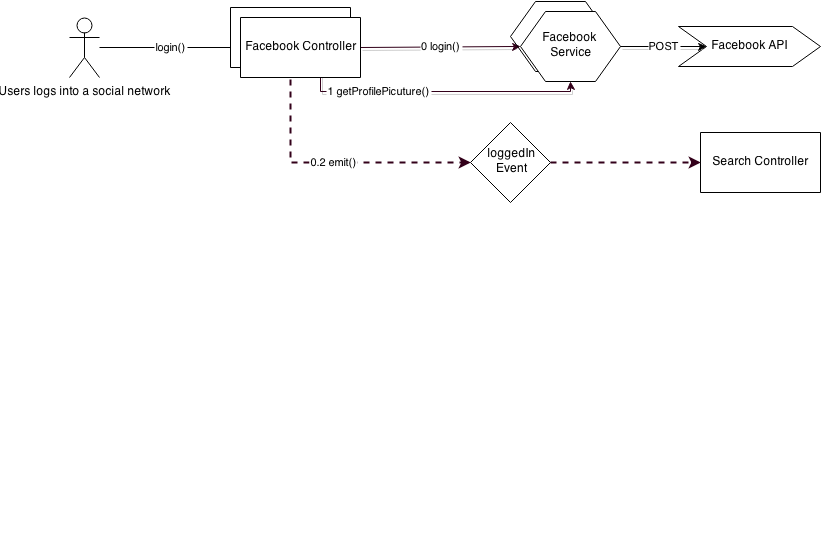
\includegraphics[width=\textwidth]{./img/1_login_flow}
		\caption{A schematic overview of the control flow when a user logs in.}
		\label{fig:1:controlflowLogIn}
	\end{figure}	

\subsection{Start Stalking}
\label{ss:1:startStalking}
	\Cref{fig:1:controlflowStartStalk} shows what happens in the front end when the indicates that he has logged in into all social networks he wishes to use. 
	
	If the POST to the \t{Stalker API} fails no error is reported to the user, since it does not matter to the user if his information is added to our database. 

		\begin{figure}
			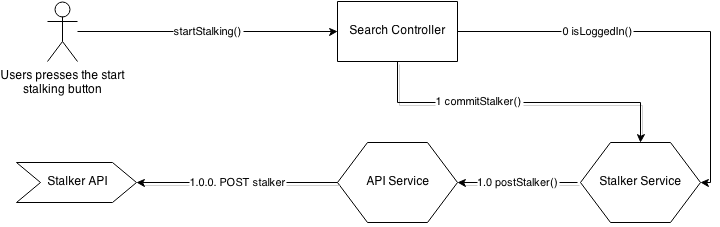
\includegraphics[width=\textwidth]{./img/1_start_stalking_flow}
			\caption{A schematic overview of the control flow when a presses the `start stalking' button.}
			\label{fig:1:controlflowStartStalk}
		\end{figure}


\subsection{Stalk}
	\Cref{fig:1:controlflowStalk} presents the flow of control when a user searches for somebody on the social networks that he has logged in to.

	The \t{Stalker Service} contains all information on the stalker. The \texttt{API Service} contains all calls to our own API, we have chosen for a separate service so that we only have to store the address of the API in one place. The Search Service broadcasts the search to the different social media controllers, in \cref{fig:1:controlflowStalk} Facebook is shown as an example. Each social network controller does a search call by calling some function in the matching service that interacts with the actual API of that social network.


	We had to use a broadcast instead of an emit as in \cref{ss:1:login} since we had to down in the scope hierarchy instead of up. \\

	We added the start stalking button to force our users to first login to all social networks they wanted to use before actually stalking somebody. This was one of the concessions we had to make due to time constraints, since this button ensures that we can post complete stalkers, instead of having to update a stalker every time he adds a social network. 

		\begin{figure}
			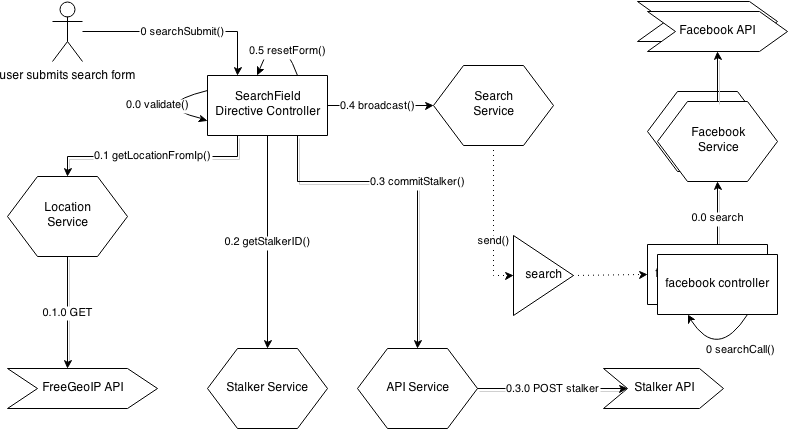
\includegraphics[width=\textwidth]{./img/1_stalking_flow}
			\caption{A schematic overview of the control flow when a user stalks somebody.}
			\label{fig:1:controlflowStalk}
		\end{figure}	

\subsection{Select Victim}
	\Cref{fig:1:controlflowVictim} shows the control flow in the front end when a user indicates that one of the found results was his victim. Even tough it does not matter to the user if the addition of his victim to our database has been reported we report success, and failure, since the user has no feedback on his actions otherwise. 

		\begin{figure}
			\missingfigure{Control flow of choosing a victim}
			\caption{A schematic overview of the control flow when a user selects somebody as his victim.}
			\label{fig:1:controlflowVictim}
		\end{figure}		

\subsection{View Statistics}
	The control flow when a user views statistics is presented in \cref{fig:1:controlflowStat}.

	\todo{Begeidend verhaaltje schrijven}

	\begin{figure}
		\missingfigure{Control flow of statistics}
		\caption{A schematic overview of the control flow of requesting the statistics and showing them to the user.}
		\label{fig:1:controlflowStat}
	\end{figure}